

\begin{figure*}[ht]
  % \vspace{-8pt}
   \begin{minipage}[b]{0.48\textwidth}
  % \begin{center}

    \subfigure[Aligned MHC pangenome]{
      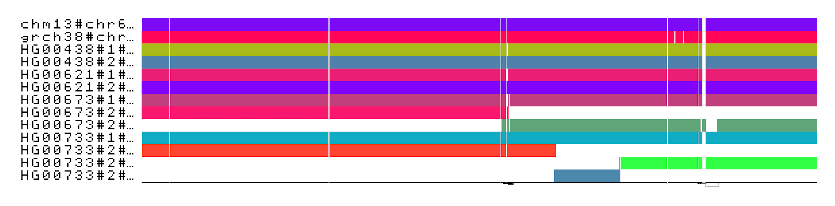
\includegraphics[width=\textwidth]{fig/mhc-align.eps}
      \label{subfig1}
    }
    \vspace{-11pt}
    \newline
    \subfigure[Consensus MHC pangenome]{
      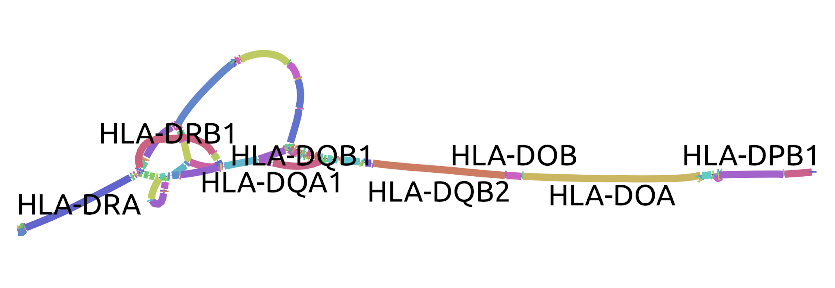
\includegraphics[width=\textwidth]{fig/mhc-pangenome.eps}
      \label{subfig2}
    }
            \caption{(b) Visualizing the Major Histocompatibility Complex
                (MHC) \textit{locus} pangenome. A) \cmd{odgi viz} 1D visualization
                of 8 haploid, phased human genome assemblies plus the chm13
                and GRCh38 reference genomes. Graph nodes’ are arranged
                from left to right. The colored bars represent the
                linearized renderings of the embedded paths versus the nodes
                in a binary matrix. The black lines under the paths are the
                links, which represent the graph topology. B)
                Bandage~\citep{26099265} representation of the graph
                topology of a consensus MHC pangenome graph representing
                only variations bigger than 100 bps. Gene labels were
                applied exploiting \cmd{odgi position} to liftover gene
                coordinates from the full graph into the consensus graph.  }

  % \end{center}
  \end{minipage}
\end{figure*}
